\documentclass{article}
\usepackage[utf8]{inputenc}
\usepackage{tikz}
\usetikzlibrary{positioning}
\usetikzlibrary{shapes}

\begin{document}

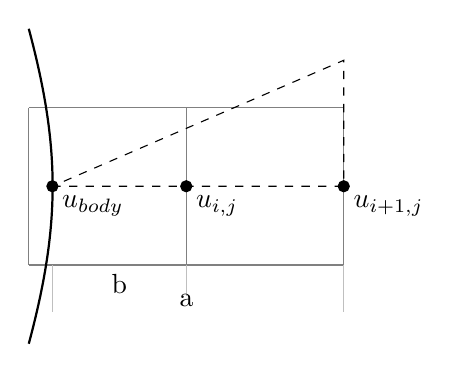
\begin{tikzpicture}
%grid
%horizontal
\draw[gray, thin] (-2,1) -- (2,1);
\draw[gray, thin] (-2,-1) -- (2,-1);
%vertical
\draw[gray, thin] (-2,1) -- (-2,-1);
\draw[gray, thin] (0,1) -- (0,-1);
\draw[gray, thin] (2,1) -- (2,-1);
%body
%\draw[black, thick] (-0.2,-1.1) -- (-0.2,1.1) node[anchor=south] {body}; 
\draw[black, thick]    (-2,-2) to[out=75,in=-75] (-2,2);
%triangle
\draw[black, dashed] (-1.7,0) -- (2,0) -- (2,1.6) -- cycle;
%nodes
\filldraw [black] (2.0,0) circle (2pt) node[anchor=north west]{$u_{i+1,j}$}; %fluid
\filldraw [black] (0,0) circle (2pt) node[anchor=north west]{$u_{i,j}$};%hybrid
\filldraw [black] (-1.7,0) circle (2pt) node[anchor=north west]{$u_{body}$};%hybrid
%vertical ticks
\draw[lightgray, thin] (-1.7, -1) -- (-1.7, -1.6);
\draw[lightgray, thin] (0, -1) -- (0, -1.4);
\draw[lightgray, thin] (2, -1) -- (2, -1.6);
%distance markers
\node[anchor=north] at (-0.85, -1) {b};
\node[anchor=north] at (0, -1.25) {a};


\end{tikzpicture}
\end{document}